\section{Query Compilation}
In this section we describe the core compilation mechanisms applied to map and
relational polynomials. Our compilation algorithm proceeds by recursively
applying a basic compilation step. The basic compilation step applies in two
phases, first deriving a \textit{delta} query to an input query, followed by
simplification of the delta query. 

\begin{figure*}[htbp]
\begin{center}
\begin{tabular}{|l|c|l|}
\hline
Compilation procedure & Method & Example \\
\hline Precompilation i:            & $flatten$
& in: $\algsum_{1}(R(A,B) \wedge \phi(>,A,4*
           \algsum_{C}(S(C,D) \wedge \phi(>,B,D))))$
\\
bigsum rewriting & & out: $\sum_{bigsum\_A, bigsum\_B}{\algsum_{g} (\phi(>,bigsum\_A, f))}$
\\
& & where $f = 4* \algsum_{C}(S(C,D) \wedge \phi(>,bigsum\_B,D))$
\\
& & and $g = \algsum_{1}(R(A,B) \wedge \phi(=,A,bigsum\_A)
           \wedge \phi(=,B,bigsum\_B))$
\\
\hline Precompilation ii:  & $build\_poly$
& in: $3 * (\algsum_{A*D}(R(A,B) \wedge S(C,D)) + \algsum_{1}(T(E,F)))$
\\
polynomial construction &
& out: $3*\algsum_{A*D}(R(A,B) \wedge S(C,D)) + 3*\algsum_{1}(T(E,F))$
\\
\hline Delta transformation        & $delta$
& in:
    $ 3*\algsum_{A*D}(R(A,B) \wedge S(C,D)) +
     3*\algsum_{1}(T(E,F))$
, delta: $\Delta_{+R(a,b)}$
\\
& & out:
    $3*\algsum_{A*D}(\{\tuple{a,b}\} \wedge S(C,D))$
\\
\hline Aggregate simplification i:  & $simplify$
& in: $3*\algsum_{A*D}(\{\tuple{a,b}\} \wedge S(C,D))$
\\
factorization & & out:
    $3*\algsum_{A}(\{\tuple{a,b}\})*\algsum_{D}(S(C,D))$
\\
\hline Aggregate simplification ii: & $simplify$
& in: $3*\algsum_{A}(\{\tuple{a,b}\})*\algsum_{D}(S(C,D))$
\\
bound variable propagation & & out:
    $3*a*\algsum_{D}(S(C,D))$
\\
\hline Aggregate extraction        & $extract\_aggregates$
& in: $3*a*\algsum_{D}(S(C,D))$
\\
(recursion auxiliary) & & out: $\algsum_{D}(S(C,D))$
\\
\hline
\end{tabular}
\vspace{-3mm}
\caption{Summary of transformations performed during recursive compilation, to
show the input and output of each transformation. For a complete walkthrough see
the VWAP compilation example.}
\label{fig:methodsummary}
\end{center}
\end{figure*}


\feature{Delta Query Derivation}
In \compiler, a \textit{delta} refers to an insertion or deletion of a single
tuple to a relation that arrives on an update stream. A delta corresponds to a
binding of a relation's variables to constants at runtime. We denote an
insertion delta to a relation $R(A,B)$ as $\Delta_{+R(a,b)}$ (similarly
$\Delta_{-R(a,b)}$ for deletion), where $\{\tuple{a,b}\}$ describes the values
present in an update stream tuple. As an overview, \compiler\ replaces the
appropriate relations with the new delta's bound variables, and unifies these
bound variables to produce a delta query that is simpler in nature than the
original query.
Here is an example of the result of a delta transform:
\begin{align*}
\Delta_{+R(a,b)} \algsum_{A}(R(A,B) & \wedge S(B,C)) =\\
& \algsum_{a}(S(B,C) \wedge \phi(=,b,B))
\end{align*}
\noindent~Above we have eliminated one input relation to the join
with a single tuple, and propagated the bound variables $a,b$ throughout the
term.  We now describe the transformations performed with deltas on both map
terms and calculus formulae in more detail.


Figure~\ref{fig:deltarules} presents delta transformations for a semiring, which
applies to both semirings of map terms and relational calculus formulae. The
figure also describes deltas of basic map terms, which is straightforward for
constants and variables, while for sum aggregates, we sum the combinations of
how we may apply deltas to the aggregate argument and relational part.
The interesting case is for a constraint-only aggregate, whose value can
arbitrarly change despite conjunctive monomials. This is based on the insertion
and removal of tuples in the result set, when considering a constraint-only
aggregate as a conditional. There are three cases:
i) rows whose new value satisfy the condition are
  incremented by the delta query value;
ii) rows whose new value satisfy the condition, but did not previously, must
  be added to the result set (note that these rows are a subset of those
  incremented by the delta query value in the previous case);
iii) rows which previously satisfied the condition but do not any more, must be
  removed from the result set, according to the old value they contribute.

Finally, we come to deltas for relational calculus formulae. The main point to
note is that the delta for a constraint is only defined for non-nested
constraints, that is when then map term arguments in the constraint have a
zero-valued delta. \compiler\ explicitly flattens queries to ensure this
property, lifting such constraints whenever possible, otherwise transforming to
a constraints-only aggregate, which can then be handled with the appropriate map
term delta transformation. We return to the flattening process in the section on
nested query compilation.


\feature{Aggregate Simplification}
Following delta query derivation, we simplify the resulting map term by
exploiting variables bound by the delta. In short, delta bound variables, which
are constants supplied from a tuple at runtime, enable constraint
simplification, via variable unification, resulting in the propagation of delta
bound variables throughout maps and relational calculus. Map terms on which no
further bound variable propagation may be applied are used for query
evaluation. We describe this in more detail.

Given an aggregate term $\algsum_{f}(r)$, our simplification process applies in
two phases. First we identify equality constraints in the relational part of the
aggregate $r$, constructing a mapping from equated variable pairs by performing
variable unification. This mapping is used to perform variable substitution. Our
unification algorithm accepts a set of identities defining variables that must
be preserved in any mapping (i.e. must not appear in the domain of a
mapping). Indeed, delta bound variables are passed as identities to substitute
as many safe and unsafe variables as possible with these bound
variables.

Unification yields a map term with equality constraints corresponding
to mappings removed. 
For example, unifying the query
$\algsum_{1}(R(A,B) \wedge S(C,D) \wedge \phi(=,B,C))$
with variables $C,D$ as identities yields $\algsum_{1}(R(A,C) \wedge S(C,D))$.
However, requiring variables as identities during
unification can lead to inconsistencies -- a mapping entry that does not
preserve the required identities. Such inconsistencies must remain present in
the resulting map term.
For example, unifying
$\algsum_{1}(R(A,B) \wedge S(C,D) \wedge T(E,F) \wedge \phi(=,B,C) \wedge
\phi(=,D,E)$ with $C,D,E,F$ as identities yields
 $\algsum_{1}(R(A,C) \wedge S(C,D) \wedge T(E,F) \wedge \phi(=,D,E))$.

The mapping obtained from the relational part of the aggregate can then be used
to perform substitutions in the aggregate argument map term. We recursively
apply this simplification to any nested aggregates in constraint map terms.
At a high level, this form of aggregate simplification induces a structured
propagation of delta bound variables. Delta bound variables are propagated
top-down through a parse tree as a result of recursive application, first being
passed to the relational part of aggregates to replace safe and unsafe
variables. Subsequently aggregate simplification propagates delta bound
variables into the aggregate argument term, essentially a sideways propagation
within sibling parse trees present at aggregates.

\newcommand{\indentcode}{\hspace{5mm}}
\begin{algorithm}[htbp]
\caption{compile($db\_schema, map, params, term$)}
\label{alg:compile}
\begin{algorithmic}[1]
\IF{$\neg recursive\_call$}
  \STATE \COMMENT{Precompilation step}
  \STATE $term \leftarrow build\_poly(flatten(term))$
\ENDIF
\STATE $code \leftarrow []$
\FOR{$(relation, schema) \in db\_schema$}
  \STATE \COMMENT{Compile delta for a single relation event}
  \STATE $bound\_vars \leftarrow prefix("b\_\_", schema) \cup ext\_vars$
  \STATE $dt \leftarrow filter(\lambda x. x \neq 0, simplify($
    \STATE \indentcode $delta(ext\_maps,term),bound\_vars, params)$
  \STATE $name\_prefix \leftarrow map+relation$
  \STATE $(done, todos) \leftarrow extract\_aggregates($
    \STATE \indentcode $dt, name\_prefix, bound\_vars)$
  \FOR{$(done\_terms, done\_params) \in done$}
     \STATE $code += generate\_code(relation,$
     \STATE \indentcode $map, done\_terms, done\_params)$
  \ENDFOR
  \STATE \COMMENT{Recur for remaining terms}
  \FOR{$(next\_map, next\_params, next\_term) \in todo$}
  \STATE $code += compile(db\_schema, $
  \STATE \indentcode $next\_map, next\_params, next\_term)$
  \ENDFOR
\ENDFOR
\RETURN $code$
\end{algorithmic}
\end{algorithm}


\feature{Recursive compilation}
Together, the delta query derivation and aggregate simplification form one step
of our recursive compilation algorithm that is applied for a delta to a single
relation. 
Algorithm \ref{alg:compile} shows our algorithm for recursively compiling deltas
to produce source code. Our recursive compilation algorithm works by starting
with a flattened query, compiling deltas for all relations. This results in a
set of simplified delta map terms which we can evaluate to compute the query
result. Note that each delta map term contains one fewer input relation,
replaced with bound variables. We begin a recursive compilation step by
extracting any remaining aggregates in our delta map terms, and using these as
the new starting point for compilation. Thus by compiling again for all
relations, we obtain deltas of delta map terms, and repeat the process until the
delta map terms produced contain no relations, rather, all relations' variables
have been replaced by bound variables from deltas.

Regarding aggregate extraction, we track aggregates remaining inside delta map
terms in a list of declared maps, indicating that we will physically materialize
a datastructure to maintain the result of the aggregate. We perform a simple
deduplication to avoid creating redundant maps, since different recursive
compilation paths may produce identical maps. Finally, aggregate extraction
determines map keys or \textit{parameters}. These are the delta bound variables
from the current compilation step, that will not be available when considering a
delta to a different input relation. For example consider the query
$\algsum_{A*D}(R(A,B) \wedge S(B,C) \wedge T(C,D)$, and its delta map term
following compilation for $\Delta_{+R(a,b)}$:

\[a*\underbrace{\algsum_{D}(S(B,C) \wedge T(C,D) \wedge \phi(=,b,B)}_{m[b]}\]

\noindent~where $m[b]$ denotes the aggregate extracted into a map, and the term
to be recursively compiled. Prior to such a recursive call, the variable $b$ is
a parameter to the map, and no longer bound when considering a different
delta. Thus we replace $b$ with a fresh variable, and evaluate for each value of
$b$ (i.e. the domain of variable as defined by the map key domain). For the map
$m[b]$ above, the new term is:
$\algsum_{D}(S(B,C) \wedge T(C,D) \wedge \phi(=,B',B)$

\noindent~However often such parameters are unified given constraints in the map
term (as would happen with $\Delta_{+S(b,c)} m[b]$). Note that until we consider
nested queries, map parameters will always originate from a different
relation to that of a delta. Thus we only need to deal with expansion and
contraction of map key domains in the nested query case, and we will return to
this issue of domain maintenance and initial values computation for previously
unseen delta bound variables.

Figure~\ref{fig:methodsummary} presents an
overview of the compilation process, including these two core phases, as well as
precompilation steps and additional methods needed to recursively apply the core
compilation described here.


\begin{example}\feature{Flat query compilation example}
We now walk through compiling the following flat query, given in SQL as
\texttt{select sum(a*d) from R join S join T}:

\vspace{-3mm}
\begin{align*}
& q[] = \algsum_{A*D}(R(A,B) \wedge S(B,C) \wedge T(C,D))\\
& \hspace{-1.5cm}\mbox{\sc Compilation level 1:}\\
\Delta_{+R(a,b)} & q[] +=
a * \underbrace{\algsum_{D}(S(B,C) \wedge T(C,D) \wedge \phi(=,b,B)}_{qR[B']}\\
\Delta_{+S(b,c)} & q[] +=
\underbrace{\algsum_{A}(R(A,B) \wedge \phi(=,B,b))}_{qS1[B']} * \\
& \underbrace{\algsum_{D}(T(C,D) \wedge \phi(=,c,C))}_{qS2[C']}\\
\Delta_{+T(c,d)} & q[] +=
d * \underbrace{\algsum_{A}(R(A,B) \wedge S(B,C) \wedge \phi(=,c,C)}_{qT[C']}\\
\end{align*}

\vspace{-10mm}
\begin{align*}
& \hspace{-1.5cm}\mbox{\sc Compilation level 2:}\\
\Delta_{+S(b,c)} & \algforeach \; B': qR[B'] += \\
& \algsum_{D}(T(C,D) \wedge \phi(=,B',b) \wedge \phi(=,C,c))
 \\
\therefore \Delta_{+S(b,c)} & qR[b] +=
\underbrace{\algsum(T(C,D) \wedge \phi(=,C,c))}_{qRS[C'] = qS2[C']}
\\
\Delta_{+T(c,d)} & \algforeach \; B': qR[B'] +=  \\
& d * \underbrace{\algsum_{1}(S(B,C) \wedge \phi(=,B',B) \wedge
  \phi(=,C,c))}_{qRT[B'',C']}
\\
\Delta_{+R(a,b)} & qS1[B'] = \algforeach \; B': qS1[B'] +=
a * \algsum_{1}(\phi(=,b,B'))
\end{align*}

\vspace{-7mm}
\begin{align*}
\therefore \Delta_{+R(a,b)} & qS1[b] += a\\
\Delta_{+T(c,d)} & qS1[B'] = 0 \\
\Delta_{+R(a,b)} & qS2[C'] = 0 \\
\Delta_{+T(c,d)} & qS2[C'] = \algforeach \; C': qS2[C'] +=
d * \algsum_{1}(\phi(=,C',c))
\\
\therefore \Delta_{+T(c,d)} & qS2[c] += d\\
\Delta_{+R(a,b)} & \algforeach \; C': qT[C'] += \\
& a * \underbrace{\algsum_{1}(S(B,C) \wedge \phi(=,b,B) \wedge
  \phi(=,C,C'))}_{qTR[B',C''] = qRT[B'',C']}
\end{align*}
\begin{align*}
\Delta_{+S(c,d)} & \algforeach \; C': qT[C'] += \\
& \algsum_{A}(R(A,B) \wedge \phi(=,B,b) \wedge \phi(=,c,C'))\\
\therefore \Delta_{+S(b,c)} & qT[c] +=
\underbrace{\algsum_{A}(R(A,B) \wedge \phi(=,B,b))}_{qTS[B'] = qS1[B']}
\end{align*}

\vspace{-3mm}
\begin{align*}
& \hspace{-1.5cm}\mbox{\sc Compilation level 3:}\\
\Delta_{+S(b,c)} & \algforeach B',C': qRT[B',C'] += \\
& \algsum_{1}(\phi(=,B',b) \wedge \phi(=,C',c))
\\
\therefore \Delta_{+S(b,c)} & qRT[b,c] += 1
\end{align*}
\end{example}

\noindent The resulting code is:

\begin{Verbatim}
int q;
map<int, int> qR, qS1, qS2, qT;
map<tuple<int, int>, int> qRT;

void on_insert_R(int a, int b) {
    q += a*qR[b]; qS1[b] += a;
    foreach c in keys(qT): qT[c] += a * qRT[b,c];
}

void on_insert_S(int b, int c) {
    q += qS1[b] * qS2[c];
    qR[b] += qS2[c]; qT[c] += qS1[b];
    qRT[b,c] += 1;
}

void on_insert_T(int c, int d) {
    q += d*qT[c]; qS2[c] += d;
    foreach b in keys(qR): qR[b] += d * qRT[b,c];
}
\end{Verbatim}

We omit the code produced for handling deletions on the input stream -- the code
is analagous to the insertion code seen above with decrements to maps instead of
increments.


\subsection{Nested query compilation}
Recall the VWAP query presented in Section~\ref{sec:intro}, with the average
aggregate replaced by a sum aggregate. Note that we can simply compute the
average by computing both the sum and count aggregates, and dividing at the top
aggregation level. The \compiler\ calculus representation is:
\begin{align*}
\algsum_{P*V}( & Bids(P,V) \wedge \\
& \phi(>, 0.25*\algsum_{V1}(Bids(P1,V1)), \\
& \qquad \algsum_{V2}(Bids(P2,V2) \wedge \phi(>,P2,P))))
\end{align*}

\feature{Nested variable extraction and flattening}
\comment{
\todo{
Explain why we flatten, i.e. why there is no delta rule for constraints
with non-zero delta terms, e.g. }
\begin{align*}
\Delta_{+R(\vec{r})}\phi(\theta,f,g) & := &\\
&& \algif \phi_{new} \;\algthen\; ??? \; \algelse \; 0 +\\
&& \algif \phi_{new} + \neg \phi_{old} \; \algthen \; ??? \; \algelse \; 0 +\\
&& \algif \neg \phi_{new} + \phi_{old} \; \algthen \; ??? \; \algelse \; 0
\end{align*}

This seems to be because of no clean way to express the delta purely in terms of
parse subtrees, from the constraint -- we need to refer to parent tree nodes and
sibling nodes in the \texttt{then} part of the conditional. What if we had taken
an algebraic approach, where we have a selection operator $\sigma$? We could
then write:
\begin{align*}
\Delta_{+R(\vec{r})} \sigma_{f \theta 0}(Q) & := &
   \sigma_{f_{new} \theta 0}(\Delta_{+R(\vec{r})} Q) \cup \\
&& \sigma_{f_{new} \theta 0 \wedge \neg(f \theta 0)}(Q) - \\
&& \sigma_{not(f_{new} \theta 0) \wedge f \theta 0}(Q)
\end{align*}

The other major reason seems to be no clean separation of selections from unions
and joins, as needed by our semiring abstraction. We could have selections (and
even projections) at the top-level, and then polynomials of unions and joins as
we currently do. However, we cannot have selections at the leaves alone, due to
join predicates for example.
}
In the delta rules above, we have not defined a delta transformation in the case
where constraints contain map terms with non-zero deltas. This occurs with
scalar subaggregate queries, and in this section we describe a transformation
that \textit{flattens} out such queries when they are provided by the user, into
a constraint-only aggregate. We apply flattening as a preprocessing step, prior
to performing any compilation. Note that this flattening concerns nested queries
within constraints -- nested queries that occur as aggregate arguments are
directly handled in the delta rules described above.

Our flattening transformation is essentially a parse tree rotation operation
that separates the usage of variables in a nested fashion from their originating
relation. Flattening replacing nested variables in constraints with fresh
variables called \textit{\bigsum} variables. 
We describe by the VWAP example:

\begin{align*}
  \algsum_{P*V}( & B(P,V) \wedge \\
& \phi(<, 0.25*(\algsum_{V1}(Bids(P1,V1)),
\\
& \qquad \algsum_{V2}(B(P2,V2) \wedge \phi(>, P2, P)))) \\
= \sum_{\xi} \algsum_{f}( & \phi(<, 0.25*\algsum_{V1}(Bids(P1,V1)), \\
& \algsum_{V2}(B(P2,V2) \wedge \phi(>, P2, \xi)))) \\
\mbox{ where } f = & \; \algsum_{P*V}(B(P,V) \wedge \underline{\phi(=,P,\xi)})
\end{align*}

Above, $\xi$ is the \bigsum\ variable introduced for the nested usage of $P$,
and the underlined terms is a new constraint introduced on the bigsum variable
to ensure the original query's semantics hold. This constraint equates the
bigsum variable to the original variable that was used in nested fashion. We can
abstractly represent this transformation as:

\vspace{-3mm}
\begin{align*}
\algsum_{f}(\mathcal{R(\vec{A})} \wedge \phi[\vec{A}]) :=
\sum_{\xi} \algsum_{f^*}(\phi[\vec{A} \mapsto \vec{\xi}]) \\
 \mbox{ where} f^* = \algsum_{f}(\mathcal{R(\vec{A})} \wedge \vec{A} = \vec{\xi})
\end{align*}

\vspace{-2mm}
\noindent~where $\mathcal{R(\vec{A})}$ is a relational calculus formula that
does not contain constraints with nested aggregates, and defines safe variables
$\vec{A}$, $\phi$ is a constraint whose terms include nested aggregates and
$\phi[\vec{A} \mapsto \vec{\xi}]$ denotes the substitution of variables
$\vec{A}$ by variables $\vec{xi}$ in the map terms of $\phi$.
Note the domains of these \bigsum\ variables are also decoupled from the
original nested variables' domains, and we explicitly maintain \bigsum\ variable
domains as separate datastructures in the code generated. We will see an example
of this datastructure in the compilation walkthrough for the VWAP query.

\comment{
Any constraint in the resulting map term uses only those variables defined
within the constraint's map terms, or \bigsum\ variables. Flattening extracts
these nested constraints into a constraints-only aggregate, with an aggregate
argument term consisting of the remainder of the original map term. Thus our
flattening transformation evaluates the nested constraint for each value of the
\bigsum\ variable, and provided this condition holds, subsequently evaluates the
original map term with an additional constraint between the original nested
variable and the \bigsum\ variable.
}

\comment{
The general form of our transformation is:

\begin{align*}
\algsum_{f}( & Q(\vec{A}) \wedge \bigwedge_i \phi_i(\theta_i, g_i[\vec{A}], h_i[\vec{A}])) \\
= & \; \algsum_{
\underbrace{\algsum_{f}(Q(\vec{A}) \wedge \bigwedge_i \phi(=,A_i,\xi_i))}_{t}}(
\underbrace{\bigwedge_i \phi_i(\theta_i, g_i[\vec{A} \mapsto \vec{\xi}], h_i[\vec{A} \mapsto \vec{\xi}])}_{c})
\end{align*}
}

\feature{Domain maintenance}
In the presence of nested queries, we encounter the issue that map parameters
may take on values that we have previously not seen during lookups.  This
includes cases when both bigsum variables and group-by parameters as map
parameters.  The challenge here is that we may be required to evaluate the map
term for these new parameter values on an aribtrary database, and it is not
generally the case that the map term for these new parameter values yields zero
on an arbitrary database. We present both situations by example for a map
$m[B']$ accessed by an unseen value $b'$, starting with a map term that is equivalent to zero:

\vspace{-3mm}
\[\algsum_{A}(R(A,B) \wedge \phi(=,B,B'))\]

\noindent~Here if $b'$ corresponds to a new domain value for $B'$, we can infer
that the value does not lie in the domain fo $B$, otherwise $m[b']$ would have
been incrementally for $\Delta_{+R(a,b')}$. Thus the initial value of the map is
zero. Now consider the map term:

\vspace{-3mm}
\[\algsum_{A}(R(A,B)\wedge \phi(<, B, B'))\]

\noindent~Here the relation $R$ may indeed contain values of $B$ satisfying the
predicate, without actually containing $b'$. Thus we must ensure the map $m[B']$
is populated with the correct entry for $b'$ prior to performing a lookup. Our
current approach for this is to use a standard relational algebra plan to
compute initial values, and have implemented the generation of a plan-based
query engine in \compiler. In certain cases, we can avoid this from-scratch
computation by leveraging neigboring map entries, for example in the case of
monotonic map terms such as min and max aggregates. However a full discussion of
such optimizations for initial value computation lies outside the scope of this
paper.


\begin{example}\feature{Nested query compilation example}
We present a compilation trace for the VWAP query. First we present the
flattened form:
\begin{align*}
q[] & = \sum_{bigsum\_p}{\Big[\algif \; \phi(>, f, g) }\\
    & \algthen \; \algsum_{P*V}(Bids(P,V) \wedge bigsum\_p = P) \;
      \algelse \; 0 \Big]\\
\mbox{where } & f = 0.25*\algsum_{V1}(Bids(P1,V1))\\
\mbox{and } & g = \algsum_{V2}(Bids(P2,V2) \wedge P2 > bigsum\_p)
\end{align*}

\begin{align*}
& \hspace{-1.75cm}\mbox{\sc Compilation level 1:}\\
\Delta_{+Bids(p,v)} & q[] += \sum_{bigsum\_p} \Big[ \\
& [ \algif \; \phi(>,\underbrace{f}_{m1[]}+\Delta f, \underbrace{g}_{m2[bigsum\_p]}+\Delta g) \; \\
& \algthen \; \Delta \algsum_{P*V}(Bids(P,V) \wedge bigsum\_p = P) \;
    \algelse \; 0 ] \\
+ \; & [ \algif \; \phi(>,\underline{f}+\Delta f, \underline{g}+\Delta g) \wedge
    \neg\phi(>,\underline{f},\underline{g}) \\
& \algthen \; \underbrace{\algsum_{P*V}(Bids(P,V) \wedge
    bigsum\_p = P)}_{m3[bigsum\_p]} \;
    \algelse \; 0 ] \\
+ \; & [ \algif \; \neg \phi(>, \underline{f}+\Delta f, \underline{g}+\Delta g)
    \wedge \phi(>,\underline{f},\underline{g}) ] \\
& \algthen \; - \underline{\algsum_{P*V}(Bids(P,V) \wedge bigsum\_p = P)} \;
    \algelse \; 0
\Big]
\end{align*}

\begin{align*}
& \hspace{-1.75cm}\mbox{\sc Compilation level 2:}\\
\Delta_{+Bids(p,v)} \; & m1[] += v\\
\Delta_{+Bids(p,v)} \; & \algforeach \; bigsum\_p : \; m2[bigsum\_p] += \\
& \qquad \algif \; p > bigsum\_p \;\algthen \; v \; \algelse \; 0 \\
\Delta_{+Bids(p,v)} \; & \algforeach \; m3[bigsum\_p] += \\
& \qquad \algif \; bigsum\_p = p \; \algthen \; p*v \; \algelse \; 0\\
\therefore \; & m3[p] += p*v
\end{align*}
\end{example}

Above, the underlined terms correspond to duplicate map terms, where maps can be
reused. The code produced is:

\begin{Verbatim}
int q, m1; map<int, int> m2, m3; set<int> dom_bigsum_p;

void on_insert_bids(int p, int v) {
  dom_bigsum_p.insert(p);

  // Initial value computation
  if ( !m2.haskey(p) )
    foreach b_p, b_v in bids:
      m2[p] += (p < b_p? b_v : 0);

  if ( !m3.haskey(p) ) {
    foreach b_p, b_v in bids:
      m3[] += (p == b_p? b_p*b_v : 0);
  }
\end{Verbatim}

\begin{Verbatim}
  // Compilation level 1
  foreach bigsum_p in dom_bigsum_p:
    q += if (m1+0.25*v >
              m2[bigsum_p]+(p>bigsum_p? v : 0))
         then (p==bigsum_p? p*v : 0) else 0;
    q += if (m1+0.25*v >
               m2[bigsum_p]+(p>bigsum_p? v : 0))
             && (m1 <= m2[bigsum_p])
         then m3[bigsum_p] else 0;
    q += if (m1+0.25*v <=
               m2[bigsum_p]+(p>bigsum_p? v : 0))
           && (m1 > m2[bigsum_p])
         then -m3[bigsum_p] else 0;

  // Compilation level 2
  m1 += 0.25*v;
  foreach bigsum_p in keys(m2):
    m2[bigsum_p] += (p > bigsum_p? v : 0);
  m3[p] += p*v;
}
\end{Verbatim}


\begin{figure*}[htbp]
\begin{center}
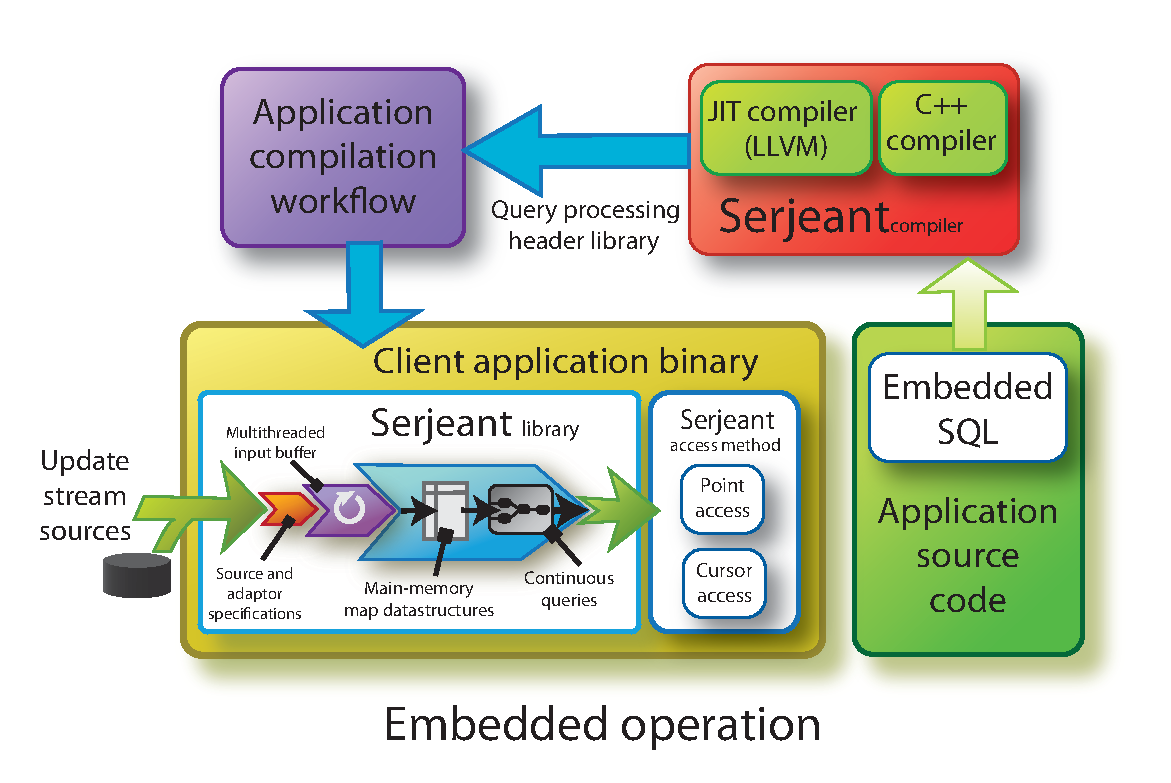
\includegraphics[scale=0.35]{figures/dbt-arch-embedded}
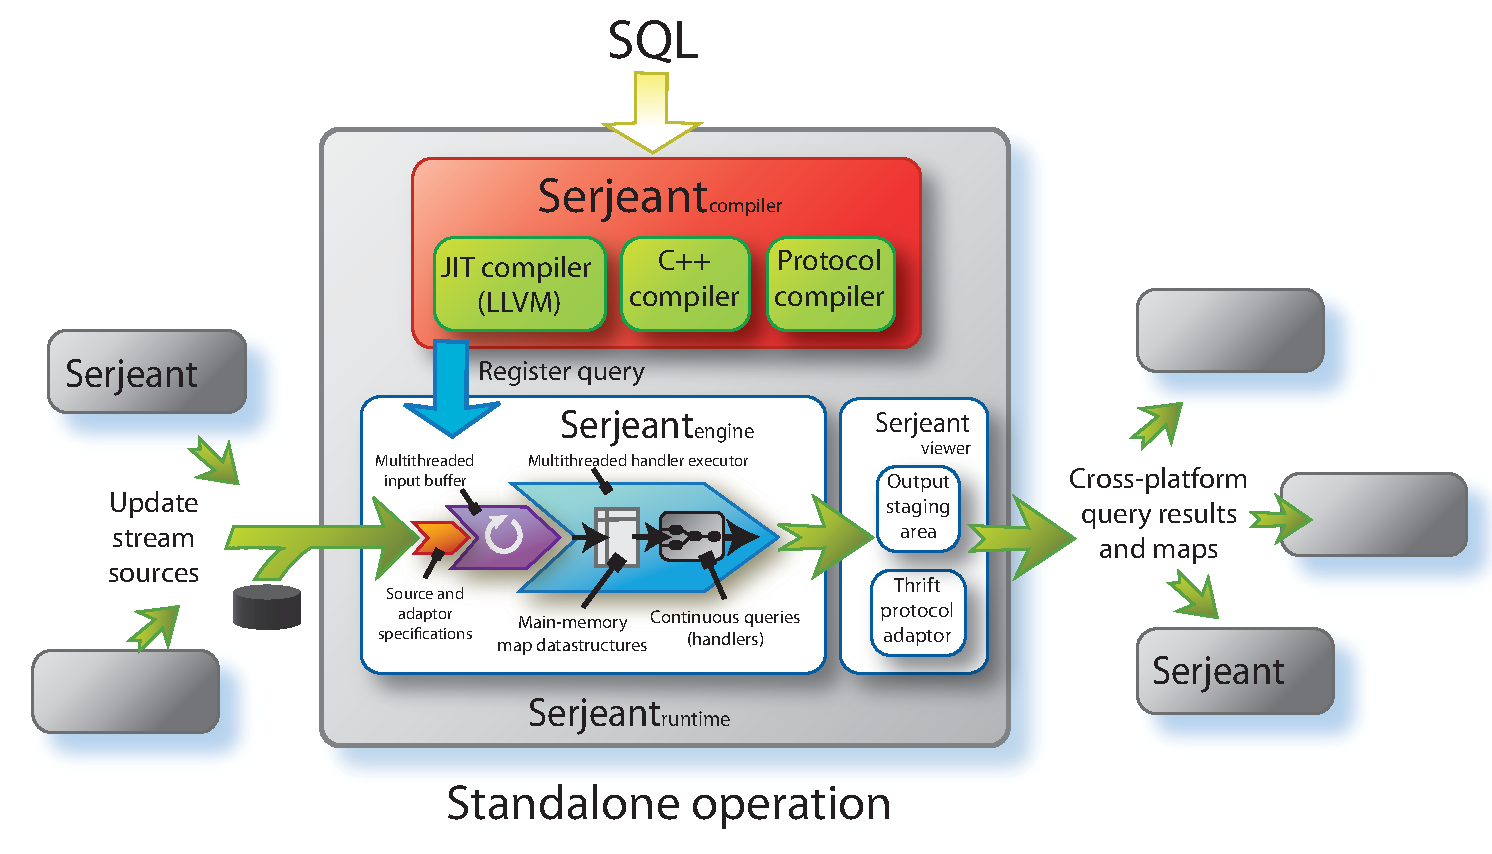
\includegraphics[scale=0.35]{figures/dbt-arch-standalone}
\end{center}
\vspace{-5mm}
\caption{\compiler\ compiled query evaluation modes: i) compilation for embedded
  query processing ii) query object compilation for use in a distributed stream
  processing engine.}
\label{fig:overview}
\end{figure*}


\comment{
\subsection{Code Generation}
Describe:
\begin{itemize}
\item accumulator language which allows simple code generation for
procedural languages such as C++/Java.
\item differences between simple accumulator language and implementations of
relational calculus which pass around sets, resulting in a larger greater
copying of data and more memory pressure. Accumulator language is even different
to pipelining query plans, which can push tuples through to an accumulator
(i.e. incr() function of an aggregate) at a tuple granularity, but still copies
data from using an operator processing model.
\end{itemize}
}